
\documentclass{article}

\usepackage[ngerman]{babel}                     %for german umlauts
\usepackage[utf8]{inputenc}
\usepackage{subfigure}
\usepackage{float}
%\usepackage[framed,autolinebreaks,useliterate]{mcode}
%\usepackage[bw,framed,autolinebreaks,useliterate]{mcode}
% \usepackage[ansinew]{inputenc}        %for german umlauts

\usepackage{listings}

\usepackage{graphicx}
\usepackage{hyperref}

\usepackage{amssymb}    %for different fonts
\usepackage{amsmath}
% Geht nicht: \usepackage{bbm}
% \usepackage[usenames,dvips]{color} %only way to get it running with pdf:(
% \usepackage[pdftex,usenames,dvipsnames]{color}        % does not work
% \usepackage{color}
\usepackage{verbatim}
\usepackage{polynom}

\setlength{\parindent}{0pt}
\addtolength{\hoffset}{-2cm}
\addtolength{\voffset}{-1cm}
\addtolength{\textheight}{3cm}
\addtolength{\textwidth}{3cm}

\newcommand{\im}{\operatorname{Im}}
\newcommand{\rg}{\operatorname{rg}}
\newcommand{\ggt}{\operatorname{ggT}}

\lstset{ %
  language=Matlab,                % the language of the code
  frame=single,                   % adds a frame around the code
  tabsize=2,
  basicstyle=\footnotesize
}

\begin{document}

\section*{\begin{center} Mustererkennung - Aufgabenblatt 08 \end{center}}
\begin{center}
  André Hacker und Dimitri Schachmann \\
\end{center}

\subsection*{1. Offline vs. Online}
	Den Code der Aufgabe 1 und 2 löst haben wir diesmal im Anhang am Ende.
	Wir haben zuerst die learnNeural Methode um Parameter itemsPerIteration erweitert,
	der den Algorithmus generalisiert.
	Übergibt man 1, hat man Online Learning, übergibt man N (Anzahl der Datensätze), hat man 
	klassiches Offline/Batch Learning. Übergibt man eine Zahl L dazwischen, wird in jeder Iteration
	ein L-Subset der Daten zufällig gewählt und für dieses die Gradienten berechnet. So erreichen
	wir maximale Flexibilität.\\
	
	Um Online und Offline Performance vergleichen zu können, betrachten wir bei Offline
	die effektiven Iterationen, also wie viele Gradienten berechnet wurden. Das ist nämlich 
	die Zahl, die ausschlaggebend für die Laufzeit ist. Bei Offline-Learning mit 100 Iterationen und 7000 Testdaten
	haben wir 700.000 effektive Iterationen.\\
	
	Außerdem haben wir eine logarithmische Skala für die Anzahl der Iterationen gewählt, um besser plotten zu können.\\
	
	Die Messergebnisse ergeben sich aus völlig unabhängigen Versuchen, weshalb sich Schwankungen (hier bei Ionen-Daten) ergeben. Wir haben also erst 1 Iteration durchgeführt, das Ergebnis gemessen, dann mit neuen zufälligen Werten gestartet, mehr Iterationen durchgeführt und wieder das Ergebnis gewertet.
	Das hätte man auch anders machen können (nur einen Versuch, und zwischendrin die Successrate berechnen). Unser Ansatz hat den Vorteil, dass die großen Schwankungen bei den Versuchen (hängen mit initialen Gewichten und lokalen Minima zusammen) auch sichtbar werden.
	
	Die Ergebnisse zeigen, dass Online-Learning effektiver ist, was auch die gängige Meinung der Literatur ist (vergleiche Bishop):
	\begin{figure}[H]
	  \begin{subfigure}
	    \centering
	    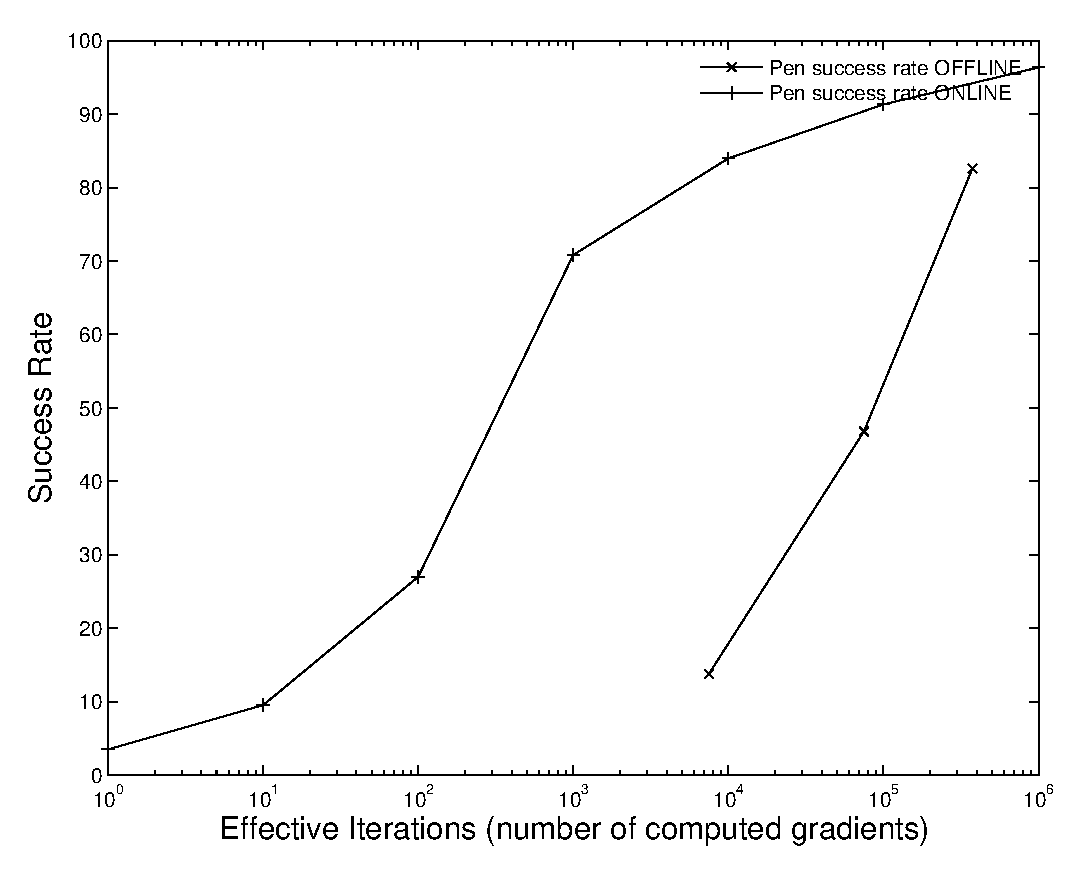
\includegraphics[scale=0.75]{task1-pen-1.eps}
      \caption{Pendigits Offline vs Online Performance}
	  \end{subfigure}
	\end{figure}

	\begin{figure}[H]
	  \begin{subfigure}
	    \centering
	    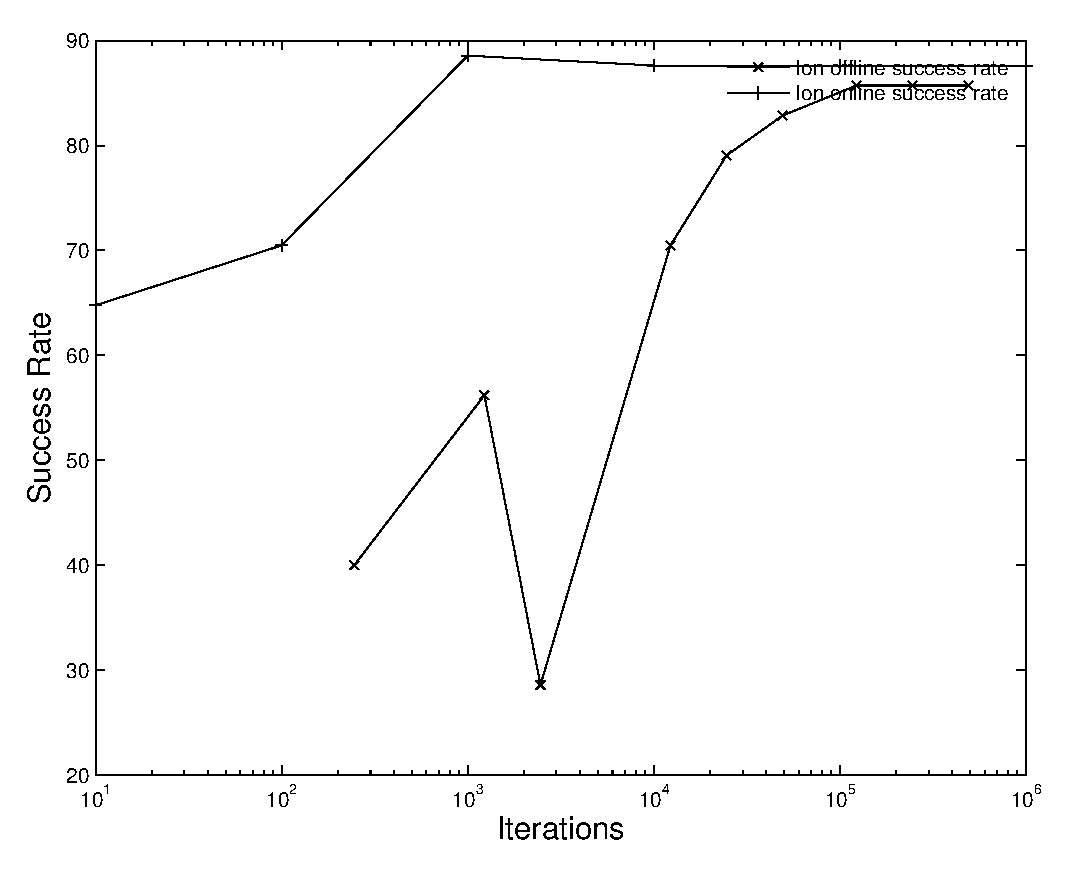
\includegraphics[scale=0.75]{task1-ion-1.eps}
      \caption{Ion Offline vs Online Performance}
	  \end{subfigure}
	\end{figure}

\subsection*{2. Rprop}
Für die implementierung des Rprop Algorithmus haben wir schlicht den
BP Code erweitert. Der learnNeural Funktion werden zusätzlich die parameter
\begin{itemize}
\item learnRateMax
\item learnRateMin
\item rprop\_u
\item rprop\_d
\item doRprop
\end{itemize}
übergeben. Wenn doRprop == 1, dann wird der Rprop Algorithmus
durchgeführt, ansonsten der gewöhnliche BP. Es ist wichtig darauf zu
achten, dass für Rprop batch learning aktiviert sein muss.

Unsere Testläufe haben ergeben, dass unsere Rprop Implementierun bei
bereits bei geringerer Iterationszahl besser ist, als BP bei der
gleichen Iterationszahl. Es war jedoch schwierig gute Konstanten zu
finden. Bei den pendigits daten war das schwieriger als bei den
Ionendaten.

Wie erwartet führt der RPROP wesentlich schneller zu guten Werten.

	\begin{figure}[H]
	  \begin{subfigure}
	    \centering
	    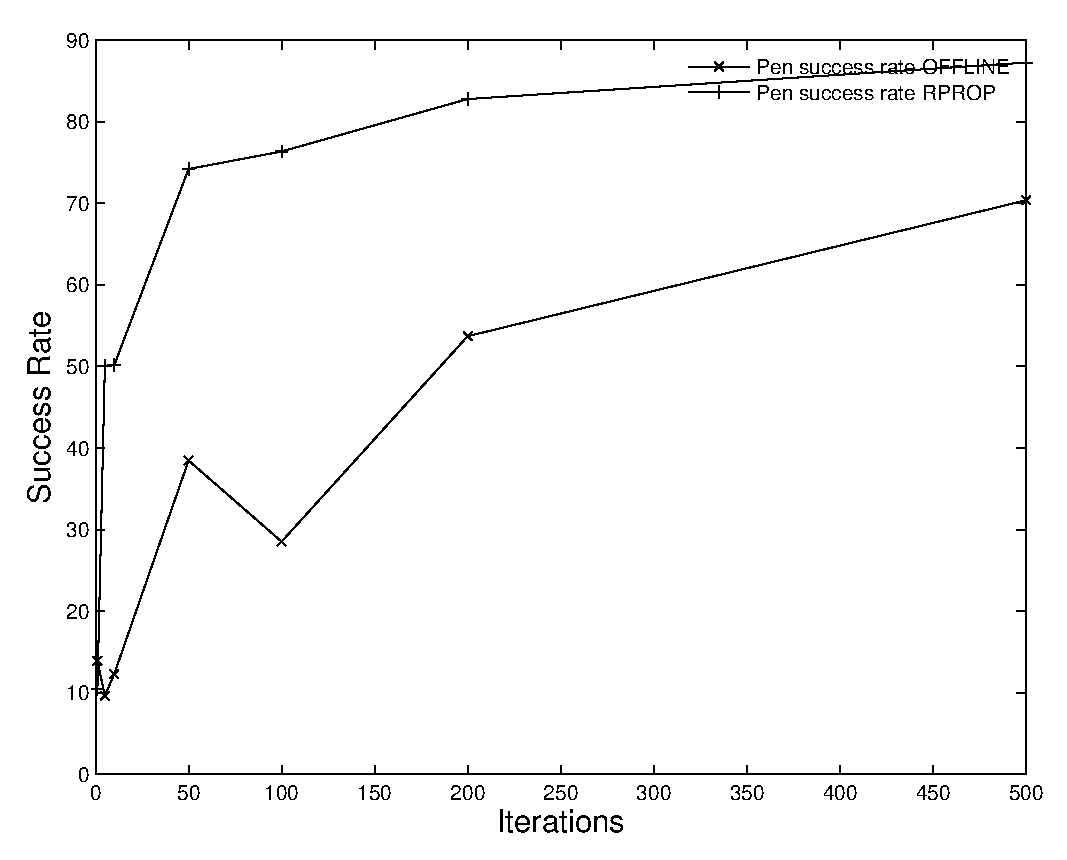
\includegraphics[scale=0.75]{task2-pen-1.eps}
      \caption{Pendigits Offline vs RPROP Performance}
	  \end{subfigure}
	\end{figure}

	\begin{figure}[H]
	  \begin{subfigure}
	    \centering
	    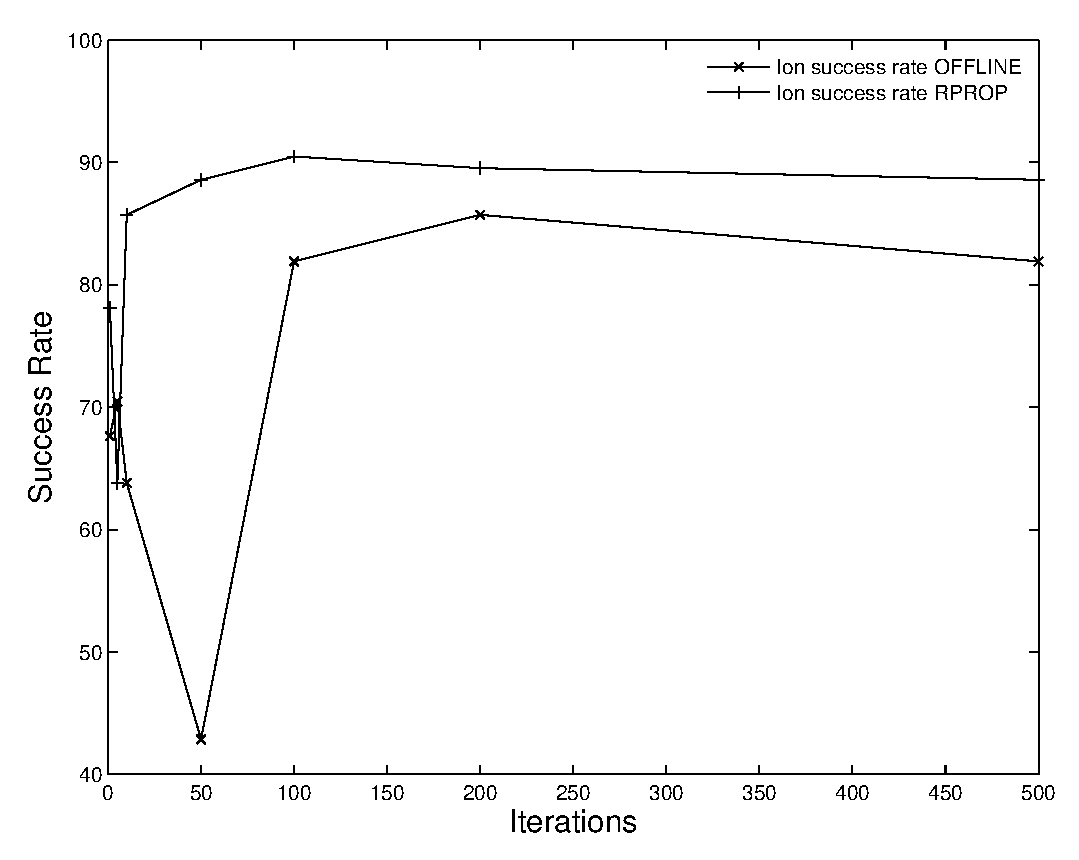
\includegraphics[scale=0.75]{task2-ion-1.eps}
      \caption{Ion Offline vs RPROP Performance}
	  \end{subfigure}
	\end{figure}

\subsection*{3. Implementierung}


	\verbatiminput{bprop.m} %a

\end{document}
